\section{Analyzing Task-Inference} \label{sec:mean_est}

To motivate further exploration of attacks on deep learning models, we present a simplified analog of multitask learning via mean estimation. Proofs of our theorems in this Section can be found in Appendix~\ref{sec:proofs}.\\ 

\noindent Suppose that there exists a set of \emph{task means} $M = \{\mu_1, \dots, \mu_T\}$ which are sampled i.i.d.\ from $\mathcal{N}(\bar{\mu}, \bar{\sigma}^2 \mathbb{I}_d)$ where $\bar{\mu}$ is the "true" mean that we would like to estimate. For each "task" $\mu_i$, we can sample $N$ (where $N$ is relatively small) points i.i.d. from $\mathcal{N}(\mu_i, \sigma^2 \mathbb{I}_d)$ and store them in the set $X_i = \{x_{i, 1}, \dots, x_{i, N} \}$. Since no individual dataset $X_i$ would yield an accurate estimate of $\bar{\mu}$ we can instead compute the sample "multitask" mean using all of the $X_i$'s as 
\[
    \hat{\mu} = \frac{1}{T}\sum_{i=1}^{T} \left( \frac{1}{N} \sum_{j=1}^{N} X_{i,j} \right)
\]

\noindent This "multitask" mean can be viewed as analogous to the weights of the shared representation in multitask learning, because we average over data, $X_i$, sampled from a mixture of Gaussian distributions, $\mathcal{N}(\mu_i, \sigma^2 \mathbb{I}_d)$, which share features, to produce an accurate estimate of the underlying common parameter, $\bar{\mu}$. We note that $\hat{\mu}$ is Gaussian with expectation and covariance

\[
\ex{\mu, X}{\hat{\mu}} = \bar{\mu} \qquad
\cov{}{\hat{\mu}} = \Big( \frac{\bar{\sigma}^2}{T} + \frac{\sigma^2}{N \cdot T} \Big) \cdot \mathbb{I}_d
\]


\begin{figure*}[t!]
    \centering
    \begin{subfigure}[c]{0.40\textwidth}  % Use [c] for center alignment
        \centering
        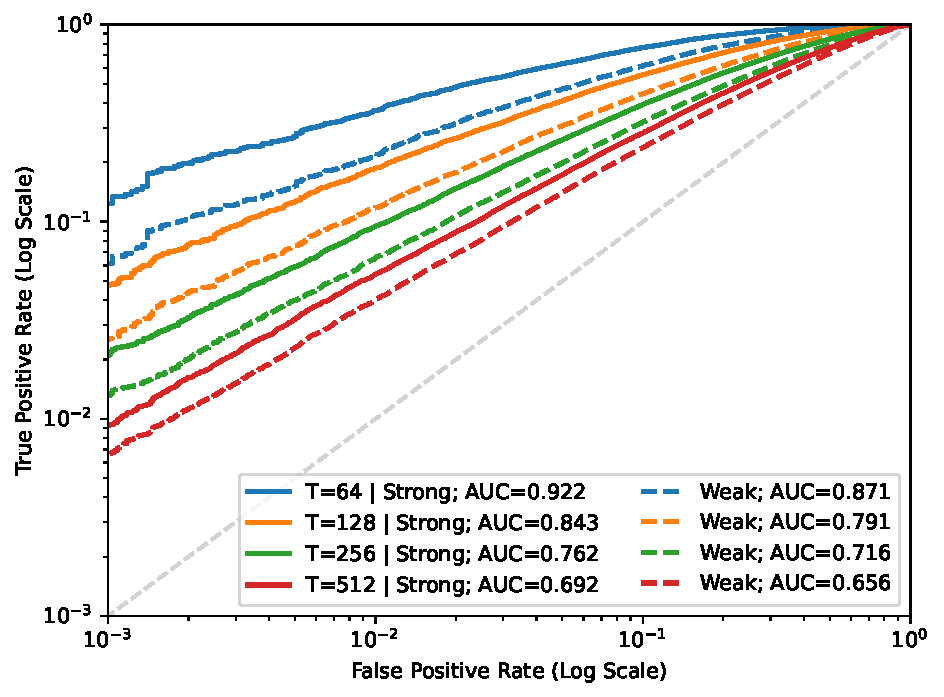
\includegraphics[width=\textwidth]{figs/mean_est_roc.pdf}
        \caption{ROC Curves for Strong and Weak Tracing Adversaries}
        \label{fig:attack_roc}
    \end{subfigure}
    \quad \quad \quad \quad \quad
    \begin{subfigure}[c]{0.45\textwidth}  % Use [c] for center alignment
        \centering
        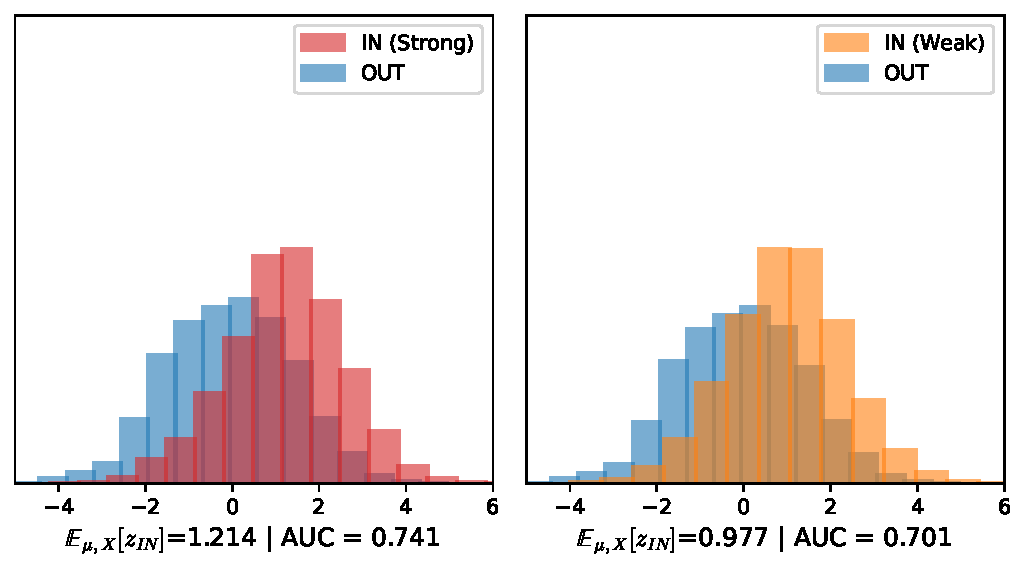
\includegraphics[width=\textwidth]{figs/mean_est_strong_v_weak.pdf}
        \caption{Distribution of Test Statistic $z$}
        \label{fig:test_statistic_mean}
    \end{subfigure}
    \caption{Results of Our Tracing Attack on Multitask Mean Estimation ( $T = 256$; $d=256$; $N=8$; $k=4$ )}
    \label{fig:mean_est_sim}
\end{figure*}


\subsection{Tracing Attack for Task Inference} \label{sec:tracing}

Here, we construct an adversary, based on prior work on tracing~\cite{dwork-2015-trace}, with similar variants to the \textbf{strong} and \textbf{weak} adversaries detailed in Section~\ref{sec:threatmodel}. We consider a challenger who releases the statistic $\hat{\mu}$ and an adversary who wants to learn whether a given task $\mu_i$ was included in the dataset that was used to compute $\hat{\mu}$.

% We assume the adversary knows the "true" mean $\Bar{\mu}$ and is given the sample "multitask" mean $\hat{\mu}$. The attack algorithm is as follows:
\noindent One possible attack would be the following:

\begin{enumerate}[labelsep=*,leftmargin=15pt]
    \item The adversary receives a challenge set, or batch of data, $B$, from the challenger where $| B | = k \leq N$, such that the samples come from a task that was used to compute $\hat{\mu}$, $\mu_{IN} = \mu_i$, or a task that was \emph{not} used to compute $\hat{\mu}$ but comes from the same underlying task distribution, $\mu_{OUT} \sim \mathcal{N}(\bar{\mu}, \bar{\sigma}^2 \mathbb{I}_d)$
    \item First, the adversary computes the sample mean of the batch
    \[
    \mu_{B} = \frac{1}{k} \sum_{x \in B}{x} 
    \]
    % which has expectation \(
    % \ex{\mu, X}{\mu_{B}} = \bar{\mu} 
    % \) and covariance \(
    % \cov{}{\mu_{B}} = \Big( \bar{\sigma} + \frac{\sigma^{2}}{k}\Big) \mathbb{I}_d
    % \)
    \item Then, the adversary computes the test statistic
    \[
    z = \inn{\hat{\mu} - \Bar{\mu}}{\mu_B - \Bar{\mu}}
    \]
    \item Lastly, the adversary performs a thresholded classification, returning $z > \gamma$ for some threshold $\gamma$
\end{enumerate}

Our adversary adapts a test statistic originally intended for membership-inference~\cite{dwork-2015-trace} that measures the correlation between the released statistic and the samples available to the adversary. However, unlike the membership-inference setting, the adversary is attempting to detect traces of the \textit{task}, or data's distribution, $\mu_i$, rather than any particular sample from one of the datasets $X_i$. In the following theorems, we find that the inclusion of a task, $\mu_i$, can be inferred by both the \textbf{strong} and \textbf{weak} adversaries, and the \textbf{strong} adversary gets a slight advantage from having access to samples in $X_i$.


\begin{thm}[Strong Adversary]  \label{thm:strong_adv}

Let $\tau$ be the index of the target task and suppose that the challenger sends the adversary a challenge set of $k$ samples $B$ such that, when the task is \textbf{IN}, the $k$ samples are drawn uniformly at random from $X_\tau$. Then the expected value of the statistic, $z$, when $\mu_\tau$ is \textbf{OUT} is 
    \[
        \ex{\mu, \: X}{z_{\textit{OUT}}} = 0
    \]
    and when  $\mu_\tau$ is \textbf{IN}, the expected value of $z$ is
    \[
        \ex{\mu, X}{z_{\textit{IN}}} = \frac{d}{T} \Big( \bar{\sigma}^2 + \frac{\sigma^2}{N} \Big)
    \]
    % \[
    %     \ex{\mu, X}{z_{IN}} = \frac{d}{T} \bar{\sigma}^{2} +  \frac{d}{NT} \sigma^{2}
    % \]
\end{thm} 


% --------------------------------------------




In Theorem~\ref{thm:strong_adv}, we see that the expectation of the \textbf{strong} adversary's test statistic, $z$, primarily grows in the dimension of the data divided by the total number of tasks used to learn the multitask mean, $\hat{\mu}$. Through this result, we demonstrate that detecting traces of tasks can be seen as a generalization of membership inference, as setting the number of tasks $T=1$, sampling $N$ datapoints, $X$, only from the single task to estimate the task mean, and allowing the adversary to use $k=1$ sample reduces $z_{IN}$ to the membership-inference test statistic, which has expectation $\Theta \left( \frac{d}{N} \right)$. In our setting, if the adversary wants to trace a single sample in the multitask mean, the expectation of their statistic would be $\Theta \left( \frac{d}{NT} \right)$. Because the total dataset size for our mean estimation is $T\cdot N$ with $N \ll T$, tracing tasks is an easier objective for the adversary than tracing individual samples, as there a larger separation between the distributions of $z_{IN}$ and $z_{OUT}$. Moreover, because the dataset is composed of multiple task distributions, a \textbf{weak} task-inference adversary can mount attacks by using data that comes from one of the included tasks but was never used in the estimation of $\hat{\mu}$.
% membership-inference.

\begin{thm}[Weak Adversary] \label{thm:weak_adv}
    Let $\tau$ be the index of the target task and suppose the challenger sends the adversary a challenge set of $k$ samples $B$ such that, when the task is \textbf{IN}, \textbf{the $k$ samples are drawn i.i.d. from the same distribution as $X_\tau$, $\mathcal{N}(\mu_\tau, \sigma^2 \mathbb{I}_d)$.} Then the expected value of the statistic, $z$, when $\mu_\tau$ is \textbf{OUT} is 0. When $\mu_\tau$ is \textbf{IN}, the expected value of $z$ is 
    \[
        \ex{\mu, X}{z_{\textit{IN}}} = \frac{d}{T} \bar{\sigma}^2
    \]
\end{thm}

Informally, Theorem~\ref{thm:weak_adv} shows that the expectation of the weak adversary's test statistic depends only on the number of tasks, and does not benefit from a smaller number of total training samples. Similar to the \textbf{strong} case, when analyzing the \textbf{weak} case, we split the statistically dependent and independent components of the sum, as the batch is drawn from the underlying task distribution for some fixed task which was included in the estimate. In contrast with the \textbf{strong} case, there is no overlap between the adversary's challenge set and the training data. Thus, we need not account for overlapping $X_{\tau,j}$'s. Rather, we only need to consider that the challenge set samples come from the same distribution, or task, as one of the tasks in the dataset used to compute $\hat{\mu}$. \\ %As shown in Theorem~\ref{thm:weak_adv}, the weak adversary's statistic only depends on the number of tasks and does not benefit from a smaller number of total training samples. \\


\begin{thm}[Variance of $z$] \label{thm:variance}
    The variance of $z$ when $\mu_\tau$ is \textbf{OUT} is
    \[
        \var{\mu, X}{z_{\textit{OUT}}} = \frac{d}{T} \Big[ \bar{\sigma}^4 + \frac{\sigma^4}{kN} + \Big( \frac{k+N}{kN} \Big) ( \bar{\sigma}^2\sigma^2 ) \Big]
    \]
    \\
    When $\mu_\tau$ is \textbf{IN}, 
    \[
        \var{\mu,X}{{z}_{\textit{IN}}} \leq {3} \var{\mu,X}{{z}_{\textit{OUT}}}
    \]
    % and
    % \[
    %     \var{\mu, X}{z_{\textit{IN}, \: \textbf{strong}}} \leq \var{\mu, X}{z_{\textit{IN}, \: \textbf{weak}}}
    % \]
\end{thm}

We note that the \textbf{strong} adversary always achieves greater attack success rates than the \textbf{weak} adversary because the distance between the expected value of the test statistic, $z$, when the task is \textbf{IN} or \textbf{OUT} is strictly larger than that of the \textbf{weak} adversary at a similar level of variance. 
%Theorem~\ref{thm:variance} shows that the correlation between $\hat{\mu}$ and the samples in the \textbf{strong} adversary's challenge set yields a slightly smaller variance than in the \textbf{weak} case.
Furthermore, this attack on mean estimation shows that the adversary's success is dependent on two distinct parts: the knowledge they receive from having \textit{member} data (i.e. the $\frac{d }{TN} \sigma^2 $ term) and the knowledge they have about the \textit{distributions}, or \textit{tasks}, that compose the dataset (i.e. the $\frac{d}{T} \bar{\sigma}^2$ term). To empirically verify our results, we simulated the attack with parameters $T = 256$, $d=256$, $N=8$, and $k=4$. The ROC curves and distribution of $z$ for both the \textbf{strong} and \textbf{weak} adversaries are shown in Figure~\ref{fig:mean_est_sim}.


\section{Methodology} \label{sec:methodology}

In this section, we realize the threat model in Section~\ref{sec:threatmodel} for machine learning models by introducing two efficient, purely black box attacks on shared representations. 

% motivate our attack by analyzing tracing attacks on a multitask analog of mean estimation, and describe our black-box attacks on multitask machine learning models. Through our analysis, we show that there is a notable separation between the success rates of \textbf{strong} and \textbf{weak} adversaries, but a task-inference adversary with \textbf{weak} access to a task's data can still infer its inclusion in the estimated mean.

\subsection{Our Task Inference Attacks}

Here, we describe two simple, purely black-box, efficient attack algorithms that are most applicable to situations where MTL is used to train a model over few samples per task (e.g. \textit{personalization}). Our attack algorithms are inspired by previous work on membership-inference attacks on image encoder models~\cite{liu2021encodermi}, where the key insight is following: For any given image, embeddings produced by well-fit encoder models are robust to augmentations, such as random rotations and horizontal flips. Computing the similarity score of the embeddings of augmentations results in a statistic that has high membership-inference signal. % We also note that prior work on 

In this work, we hypothesize that rich, shared representations learned in MTL and collaborative learning settings produce embeddings where samples from the same task exhibit both positive and negative codependencies, similar to the relationship between augmentations of the same image studied by~\cite{liu2021encodermi} and~\cite{song-2020-embeddingleakage} in the contrastive learning setting. We also believe that, in well-generalized machine learning models, some amount of correlation between samples from the same task distribution in the shared representation space exists regardless of how samples are labeled within the MTL optimization. 
% 
% In this work, we hypothesize the following: Rich representation models in a collaborative setting like MTL are not only robust to augmentations of the \textit{same} image. For a given task (or distribution) in a dataset that is composed of a mixture of tasks, samples from the same task, regardless of their labeling in the MTL optimization, have codependent embeddings in a similar way to those studied by~\cite{liu2021encodermi}. 
% We claim that samples which come from the same task have a similar relationship in representation space to the embeddings of augmentations studied by~\cite{liu2021encodermi}. Thus, our attacks aim to exploit this relationship between codependent embeddings to infer the inclusion of an entire task. 

\subsubsection{Coordinate-Wise Variance Attack (Algorithm~\ref{alg:var_attack})} To mount the \textit{coordinate-wise variance attack}, the adversary first queries the shared representation on a batch of $k$ data samples from a given task, then aggregates the embeddings into a set $E = \{ h_\theta(x_1), \dots, h_\theta(x_k) \}$. Then, the adversary computes the empirical covariance matrix of $E$ and takes the trace divided by the dimension of the embedding vectors to be the task-inference statistic, $z$. This is equivalent to computing the sum of coordinate-wise variances of the embeddings. Lastly, the adversary sets a threshold $\gamma$ such that any task with $z > \gamma$ is labeled as $IN$, and any task with $z < \gamma$ is labeled as $OUT$.

\begin{algorithm}[H]
    \caption{Coordinate-Wise Variance Attack}
    \label{alg:var_attack}
    \begin{algorithmic}[1]
       \State {\bfseries Input:} A shared representation $h_\theta$, a challenge set  $X_\tau$
       \State $E = \{ \}$ 
       \For{$x_{i} \in X_\tau$}
           \State $e_i \gets h_\theta(x_i)$ \Comment{Query representation on challenge set}
           \State $E \gets E \cup \{ e_i \}$
       \EndFor
       \State Compute $Q$, the empirical covariance matrix of $E$
       \State \Return $tr(Q)$ \Comment{Return avg.\ coordinate-wise variance}
    \end{algorithmic}
\end{algorithm}


\subsubsection{Pairwise Inner Product Attack (Algorithm~\ref{alg:inner_attack})} For our second attack, we once again use the fact that the shared representation produces close embeddings for data from the same task, but we measure similarity of the entire embedding vectors rather their individual coordinates by taking their \textit{inner products}. As in the previous attack, the adversary first queries the shared representation and aggregates the embeddings $E$. Then, for each unique pair of data samples $(x_i, x_j) \: i \neq j$, the adversary computes the absolute value of the inner product of their embeddings, $z$, and stores the value in a set $S$. The adversary then takes the mean of the $z$'s ($\Bar{S}$) and applies a threshold $\gamma$ as in the variance attack. Alternatively, the adversary can compute the normalized inner products, or \emph{cosine similarities}, of each pair of embeddings. In our evaluation, cosine similarity yields better attack performance on language models, while the standard inner product attack achieves higher true positive rates on vision models.




\begin{algorithm}[H]
    \caption{Pairwise Inner Product Attack}
    \label{alg:inner_attack}
    \begin{algorithmic}[1]
       \State {\bfseries Input:} A shared representation $h_\theta$, a challenge set  $X_\tau$
       \State $E = \{ \}$ 
       \For{$x_{i} \in X_\tau$}
           \State $e_i \gets h_\theta(x_i)$ \Comment{Query representation on challenge set}
           \State $e_i 
           \gets W (e_i - \bar{e}) $ \Comment{Apply whitening}
           \State $E \gets E \cup \{ e_i \}$ \Comment{Store normalized embedding}
       \EndFor
       \State $S = \{ \}$
       \For{all unique pairs $(e_i, \: e_j); \: i \neq j; \: e_i, e_j \in E$}
           \If{\texttt{use\_cosine\_similarity}}
               \State $(e_i, e_j) \gets \left( \frac{e_i}{\| e_i \|}, 
               \: \frac{e_j}{\| e_j \|} \right)$
           \EndIf
           \State $z \gets \vert \inn{e_i}{e_j} \vert$
           \State $S \gets S \cup \{ z \}$
       \EndFor
       \State \Return $\Bar{S}$ \Comment{Return average pairwise inner product}
    \end{algorithmic}
\end{algorithm}

% Discuss embedding whitening 
\subsubsection{Normalizing Embeddings} Unlike prior work on membership-inference~\cite{shokri-2016-mi,carlini-2022-lira} and property inference~\cite{chaudhari-2022-snap, mahloujifar2022propertypoisoning} attacks that train shadow models, our task-inference adversary requires only query access to the shared representation, eliminating the need for shadow, or reference, models to calibrate the attack. While a slightly stronger adversary could construct a labeled, auxiliary dataset of known \textbf{OUT} tasks to calibrate their attack and perform a more powerful exact one-sided test, as in~\cite{carlini-2022-lira}, we find that simple thresholding is sufficient to achieve high success rates while maintaining the purely black-box aspect of the threat model. Thus, using the adversary's sampling access to task data and query access to the shared representation, we can attempt to reduce the noise in the embedding vectors by using a \textit{whitening transformation}.

Applying a whitening transformation to the embeddings transforms them into random vectors with covariance equal to the identity matrix. By doing this, we attempt to contract the axes in the the representation space that dominate our task-inference statistics. We find that whitened embeddings often provide better signal to the adversary for our inner product attack (Algorithm~\ref{alg:inner_attack}) than raw embeddings. To compute the transformation, we first estimate the covariance matrix of the embedding space by pooling all of the embeddings available to the adversary, regardless of task or inclusion in the model's training set, and computing the regularized covariance matrix $\Sigma_{reg} = (Q + \lambda \cdot \frac{tr(Q)}{d} \mathbb{I}_d)$ where $Q$ is the sample covariance matrix, $d$ is the embedding dimension, and $\lambda$ is a small constant. Once a well-conditioned $\Sigma_{reg}$ has been estimated, a common choice for the whitening transformation would be $W = \Sigma_{reg}^{-1/2}$. To ensure that the covariance estimate is not dependent on a challenge task's data, we compute whitening transformations for each of the $2T$ tasks that we input to our attack, leaving out the data from one task each time. When applying $W$ to the embeddings, we additionally center the embeddings by computing $\bar{e}$, the sample mean of \textit{all} embedding vectors. Thus, we normalize a given embedding $e$ by computing $W(e - \bar{e})$.